\documentclass[a4paper]{article}

\usepackage[a4paper,top=0.4in,left=0.4in,right=0.4in,bottom=0.4in]{geometry}
\usepackage{graphicx}
\usepackage{rotating}

\usepackage{multirow}
\usepackage{setspace}
\usepackage{float}
\graphicspath{ {./images/} }

\usepackage{caption}

\usepackage{tabularx,ragged2e,booktabs,caption}
\newcolumntype{C}[1]{>{\Centering}m{#1}}
\renewcommand\tabularxcolumn[1]{C{#1}}

\usepackage{titling}
\setlength{\droptitle}{-10em}

\title{Group Project - 7CCSMGPR \hspace{0.5 cm}Deadline Fighters}
\renewcommand\maketitlehookc{\vspace{-10ex}}

\begin{document}

{\setstretch{0.75}
\begin{center}
		\LARGE{Group Project - 7CCSMGPR}
\end{center}
\begin{center}
		\hspace{0.5cm} Deadline Fighters \hspace{0.5 cm} Final report - March 24, 2019
\end{center}


\section{Desktop client implementation}
We made a planning framework when we realized the functionality of the desktop client. We firstly mapped out implementing upload files, download files, delete files, rename files, edit files and other functions. Secondly, implementing the ability to combine available functions into one file synchronization feature. Finally, we beautified the interface and improved user experience.\\\\
In the process of implementation, the main process is divided into the following steps:\\\\




\begin{minipage}{\linewidth}
\centering
\captionof{table}{Steps of processes} \label{table:conflict}
\begin{tabular}[H]{|C{0.75cm}|C{10.5cm}|}\toprule[1.5pt]
\bf Step & \bf Process \\\midrule
1 	&  \begin{flushleft}Configure the computer to connect to AWS S3.\end{flushleft}\\\hline
2   &  \begin{flushleft}Create a new electron project.\end{flushleft}\\\hline
3   &  \begin{flushleft}Open the project, configure the Access key ID and Secret Access Key in code and make the project connect to S3.\end{flushleft}\\\hline
4   &  \begin{flushleft}Add a file selector and initially implement the function of uploading a single file to S3.\end{flushleft}\\\hline
5  	&  \begin{flushleft}Initial download of a file with a specific name.\end{flushleft}\\\hline
6   &  \begin{flushleft}Preliminary deletion of files with specific names.\end{flushleft}\\\hline
7   &  \begin{flushleft}Rename the file on the desktop client and upload it to S3.\end{flushleft}\\\hline
8   &  \begin{flushleft}Try to use E-tag and MD5 to edit the file and incrementally upload the changed part. Then compare the local file and the last modified time of the server file to upload the modified file, but it is not successful.\end{flushleft}\\\hline
9   &  \begin{flushleft}Create a folder called deadlinefighters on the local disk.\end{flushleft}\\\hline
10  &  \begin{flushleft}List all files stored on the server.\end{flushleft}\\\hline
11  &  \begin{flushleft}Add button function to every listed file.\end{flushleft}\\\hline
12  &  \begin{flushleft}Click on each individual file, jump out of the two dialogs, download and delete, and perform related operations for specific files.\end{flushleft}\\\hline
13  &  \begin{flushleft}Simplify syncing, first upload all local files then download all server files.\end{flushleft}\\\hline
14  &  \begin{flushleft}Get a list of local files and use a loop to add an upload function to each file.\end{flushleft}\\\hline
15  &  \begin{flushleft}Get a list of server files and use a loop to add a download method to each file.\end{flushleft}\\\hline
16  &  \begin{flushleft}Add upload all function and download all function to the sync function click event.\end{flushleft}\\\hline
17  &  \begin{flushleft}Add CSS.\end{flushleft}\\\hline
18  &  \begin{flushleft}Package the whole client to a desktop application.\end{flushleft}\\
\bottomrule[1.25pt]
\end {tabular}\par
\bigskip
\end{minipage}

At the step 4, upload is the first function in file synchronization system that we tried to achieve, html5 had an input method that type = \emph{file}, it would generate a file selector and users can choose a file that in the local disk. We got the element of file in the scripts and put the element in parameters, the parameters that S3 need usually are file name, file type and file content, and file should be uploaded according to the desired format what S3 provided. S3 has an upload method and when desktop sends the parameters, the server will catch and return the error or upload file successfully.\\\\

At the next step, Letao firstly added a download function and that can download a special file, like \emph{1.txt}, from server to local. Letao used \emph{fs} module in node.js, the \emph{fs} module is the file system module, which is responsible for reading and writing files, it needs to introduce \emph{fs} module in code before use, like \emph{var fs = require(“fs”)}. We got the bucket (a storage system in S3) and key (file name) of a file, stored them in a parameter and passed it to \emph{getObject} function in S3 to got the whole element of file. Then Letao used \emph{fs.writeFileSync(filename, data, [options])}, filename will give a name of file and a path that where this file will be located.

\begin{figure}[h!]
\centering
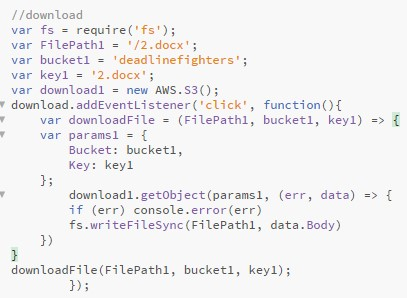
\includegraphics[scale=1.3]{code1}
\caption{download code}
\label{fig:code1}
\end{figure}

At the step 7, because S3 had no direct rename method, we only can copy a special file on the server first and give it a new name, then delete the original file.\\\\

As for \emph{edit} function, in our plan, we will handle edited files with delta synchronization. Delta sync is used to synchronize the modified portion of the file instead of re-uploading the entire file, in order to increase the speed of server processing. Delta sync relate to MD5 Algorithm and E-tag.But in the end \emph{edit} did not succeed.\\\\

Considering that the downloaded files need to be stored in a folder for users conveniently view, we tried to add a method to automatically create a folder in local. At first, Letao tried to use the \emph{FileSystemobject}, it was an object to process files and folders. But JavaScript always used \emph{ActiveXObject} to create a \emph{FileSystemObject} action file, but \emph{ActiveX} only worked on Internet Explorer. JavaScript is not allowed to access local files, but \emph{fs} module can help to deal with it. I used \emph{fs.mkdir} function to create a primary directory named \emph{deadlinefighters}. But we found the path should be set different on Mac and Windows system, Siva used \emph{navigator.platform} to check what kind of system it is and add diverse formats to build path of folder.\\\\


In order to better displayed the files on the server, we designed to list all the files. We used \emph{jQuery} to simplify code, firstly, used \emph{listObjects} function which S3 was provided to list all the files in the backstage. Then, got the key (file name) and rendered it to the front-end interface. \emph{\$.each(objects, function(i, content)} is used for traversing the array, the array here is objects, which contained all the file contents, content represents each file, content.Key shows the name of each file.\\\\

\begin{figure}[h!]
\centering
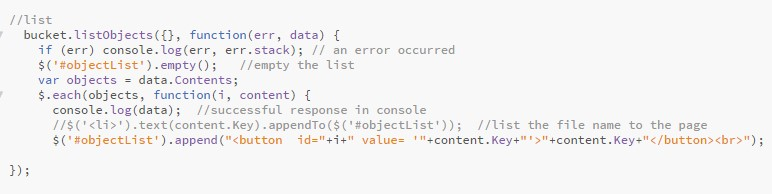
\includegraphics[scale=1.2]{code2}
\caption{download code}
\label{fig:code2}
\end{figure}

Letao changed each line of file to a button and that was convenient to add click events for download and delete functions later.\\\\
Letao set two dialogs to one file, one was download function, the other was delete function. The download function was similar with the previous code, key and file path need to be change, just passed the file values obtained by clicking the button to them. The file following represented key and got the corresponding file object from dialog, the file path pointed to the newly created folder.\\\\

\begin{center}
\emph{var file = \$(this).val();}\\\\
\emph{var filePath = '/deadlinefighters'+'/' + file;}
\end{center}

The delete function is something different, when the server file is deleted, the local file will be deleted too. Therefore, Letao added a loop algorithm to traverse local files for each deleted server file, when the name of the local file is equal to the name of the server file, the local file will also be deleted.

\begin{figure}[h!]
\centering
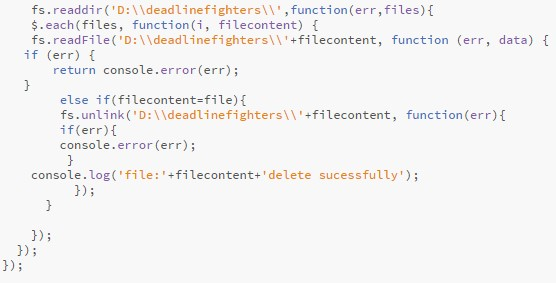
\includegraphics[scale=1.2]{code3}
\caption{download code}
\label{fig:code3}
\end{figure}

Because the files existed under a specific folder, it needed to first specify to the folder directory and then used the loop to get information about each file. At first, when read each file’s name, Letao didn’t add the \emph{“'D:$\backslash$$\backslash$deadlinefighters$\backslash$$\backslash$'+”} before\\\\

However, the result returned an error, \emph{filecontent} represented all the data in a file, not only a name, so it can’t compare with the file name in server.\\\\

The step 13 to 16 mainly completed a simple synchronization function. \emph{Upload all} and \emph{download all} functions were all involving loop. \emph{Upload all} was similar with \emph{delete}, just added an upload method to the file loop. \emph{Download all} was unlike with local file loop, the method used here is to loop through the server's files and add the download method.\\\\

In general, the desktop client of the file synchronization system has the following buttons and functions:\\\\


\begin{minipage}{\linewidth}
\centering
\captionof{table}{Buttons and functions} \label{table:conflict}
\begin{tabular}[H]{|C{2 cm}|C{9.5 cm}|}\toprule[1.5pt]
\bf Button & \bf Function \\\midrule
sync 	&  \begin{flushleft}\item{Upload all files from a local folder to server.}\item{Download all files from server to local folder.}\end{flushleft}\\\hline
upload   &  \begin{flushleft}Upload another one file from local to server.\end{flushleft}\\\hline
each line of file   &  \begin{flushleft}List each line of file in server.\end{flushleft}\\\hline
download   &  \begin{flushleft}Download one file.\end{flushleft}\\\hline
delete  	&  \begin{flushleft}Delete one file.\end{flushleft}\\

\bottomrule[1.25pt]
\end {tabular}\par
\bigskip
\end{minipage}



\section{Evaluation}
Comparing the design part to the implementation part, here is a table of what design functions are worked and what are not:\\\\



\begin{table}[h]
\caption{Priority of operations}
\centering
\begin{tabular}{|c|p{8cm}|p{2cm}|}
\hline
Operation & Object & Whether it is completed \\
\hline
\multirow{2}{*}{Upload}&{One file (May not in the local sync folder)}&Yes\\
\cline{2-3}
&All files in the local sync folder&Yes\\
\cline{1-3}
\multirow{2}{*}{Download}&{One file}&Yes\\
\cline{2-3}
&All files&Yes\\
\cline{1-3}
\multirow{2}{*}{Delete}&{One file}&Yes\\
\cline{2-3}
&All files&No\\
\cline{1-3}
\multirow{2}{*}{Rename}&{One file}&Yes\\
\cline{2-3}
&Two or more files&No\\
\cline{1-3}
\multirow{2}{*}{Edit}&{One file}&No\\
\cline{2-3}
&Two or more files&No\\
\cline{1-3}
\multirow{1}{*}{Synchronize}&{All files in the server and local syn folder}&Yes\\

\bottomrule
\end{tabular}
\end{table}

As for the desktop client, the \emph{edit} function was not worked. At the beginning, we planned to use the incremental synchronization to handle the files which were changed contents, it means not uploading the whole files but only uploading the part that are different with the original files. We planned to use MD5 to calculate file’s value and transfer the MD5 value to the server, the server determines whether the value of \emph{MD5} is different from the original file.\\\\
At first, Letao tried to use the \emph{MD5} API of \emph{node.js}, but got a problem when detecting the \emph{MD5} value of the local file, because JavaScript as a web language, it has no access to check all the parts of local files.\\\\
Then, we tried to use last modified time of files to substitute \emph{MD5}, if the last modified time of local file was different with that on server, the file would be re-uploaded. However, desktop client and mobile client both got some problems with database. For the desktop client, we tried to build a database table of file name and last modified time to store files’ information on server, but there was a problem that at the beginning, our desktop client use sync = upload all files on local + download all file on server, therefore, the last modified time always be changed. For the mobile client, the last modified time on server had different format with that on local and had an impact on the comparison of the two sides.\\\\
The second part that we not completed was conflicts. At this moment, the Android client only can connect with the S3, not the server application, so the conflicts cannot be solved temporarily. We used Amazon S3 at first, but we found S3 had their own methods to solve conflicts, so we changed to \emph{@be/http-service} to build local server.\\\\
There are the processes that we did well. Our steps were from simple to difficult, like first upload only one file then upload plenty of files in one folder at the same time. The organized steps made our project had a clear structure. \\\\
The \emph{upload all} function finally can work automatic, that means the files be added to the \emph{deadlinefighters} folder can be automatically uploaded to server.\\\\
Our desktop client can run on different computer system, like Mac or Windows. It has a strong adaptability.\\\\



\medskip

{\setstretch{0.75}

\section{Test}

In the project, our team conducted a black box test on the file synchronization tool. At the beginning, our team tested the transmission of different kinds of file names and file formats. As shown below (Table Black box test result at the beginning). As you can see from the table, we have file names under different language specifications, file names with special symbols, and different types of file formats, such as zip, png, and docx etc. used to do the upload, download, delete and rename function tests. For the uploading, downloading and deleting of files, all the objects we tested can be implemented successfully. However, for the rename function, file names with Chinese names and special symbols cannot be renamed. \\\
At the end of the project, our system implemented automation synchronize function, and these files with Chinese names and special symbols finally achieved in rename function. We analyzed the reason why we couldn't achieve it before because the name of the renamed file needs to be written in the code when we originally developed the product function, and the name with Chinese characters may be inconsistent with the language environment in which the code is written. So, the function cannot be achieved.\\\
Furthermore, we also learned and configuration test environment of Mocha, Chai and Sinon for the desktop application. We try to implement the jsunit test. But for some reasons, it is not complete.\\\

For the desktop client, we found some issues in the test.\\
For the special symbol file we have meet some issues:\\
\begin{itemize}
\item{Pdf file with(“space” “-” "'") can download but not open. Mostly can open.}
\item{ File name with "'" can be deleted in the local folder but cannot be deleted by using the delete button.}
\item{File with special symbol(*&) can upload but cannot download.}
\item{Irregular naming: \/:*?”<>|, the computer system will show that when we go to rename the file.}
\item{In addition to non-standard named symbols, file names with special symbols cannot be renamed, but a new file is uploaded.}
\end{itemize}

Besides, for the file name with Chinese we also have two issues:\\
\begin{itemize}
\item{Upload from local/download from aws file meet JSON issue because of Chinese word}
\item{Two or more files cannot be deleted, uploaded}
\end{itemize}

The .zip formatted file can be download to local folder from server but it is damaged.



Test case is show below:\\
\begin{table}[H]
\caption{Test Case}
\centering
\begin{tabular}{|p{2.5cm}|c|c|c|c|c|c|}
\hline
File & \multicolumn{3}{|c|}{Desktop} &\multicolumn{3}{|c|}{Android} \\
\hline
& upload & download & delete & upload & download & delete \\
\hline
Test.txt & T & T & T\\
\hline
123.docx & T & T & T\\
\hline
测试.pdf& F & F & F\\
\hline
!,,!.jpg & T & T & T\\
\hline
测试test.gif& F & F & F\\
\hline
Test!!!.png & T & T & T\\
\hline
123.mp3& T & T & T\\
\hline
2019df.mp4 & T & T & T\\
\hline
!,,!.zip  & T & F & T\\
\hline
Hello.rar& T & T & T\\
\hline
Test!!!.exe& T & T & T\\
\hline
Test.html& T & T & T\\
\hline
2019df.js& T & T & T\\
\hline
'!,,!'.ppt & T & F & F\\
\hline
test123.db & T & T & T\\
\hline
\bottomrule
\end{tabular}
\end{table}

\begin{table}[H]
\caption{Test Case}
\centering
\begin{tabular}{|p{2.5cm}|c|c|c|c|c|c|}
\hline
File & \multicolumn{3}{|c|}{Desktop} &\multicolumn{3}{|c|}{Android} \\
\hline
& Rename to & Rename result & Edit & Rename to & Rename result & Edit  \\
\hline
Test.txt & 123.docx & T & T\\
\hline
123.docx & 测试.pdf& F & T\\
\hline
测试.pdf& !,,!.jpg & F & F\\
\hline
!,,!.jpg & 测试test.gif & F & T\\
\hline
测试test.gif& Test!!!.png & F & F\\
\hline
Test!!!.png & 123.mp3 & T & T\\
\hline
123.mp3& 2019df.mp4 & T & T\\
\hline
2019df.mp4 & !,,!.zip  & T & T\\
\hline
!,,!.zip  & Hello.rar & F & T\\
\hline
Hello.rar& Test!!!.exe & T & T\\
\hline
Test!!!.exe & Test.html & T & T\\
\hline
Test.html& 2019df.js & T & T\\
\hline
2019df.js& '!,,!'.ppt & T & T\\
\hline
'!,,!'.ppt & test123.db & F & T\\
\hline
test123.db & Test.txt & T & T\\
\hline
\bottomrule
\end{tabular}
\end{table}

\section{System Overview}
\subsection{Brief Introduction of System Function}
With the increasing popularity of network technology and the importance of information construction, people increasingly need a file synchronisation tool to help them get the file they want on different devices. File synchronisation tools make it possible to edit the same files across multiple computers in a sensible way. This system is a ‘hub and spoke’ file synchroniser which have a single central server (the ‘hub’) to which multiple other clients (the ‘spokes’) synchronise. Developing such a tool can bring a lot of convenience to the users as it can let them get the files they need, anytime, anywhere.\\\\
Therefore, our team, \emph{Deadline Fighters}, are aims to develop a multi-host file synchronizer which can:
\begin{itemize}
\item{Allow upload and download of files from a central server (hub) through client applications with necessary authorization.}
\item{Automatically synchronize changes made by client applications unto the corresponding copy of the file in the server.}
\item{Handle all possible conflict/non-conflict scenarios of file synchronization (ie. combinations of Create, Edit, Rename, Delete) involving multiple client applications.}
\item{Enable file synchronisation through both desktop (all platform) and mobile (Android) clients.}
\end{itemize}
as we set in the initial report.\\\\
Through the outline of initial report, we detailed each function. Therefore, the file synchronisation tool that our team aim to develop will achieve the following functions as designed during the process: Upload a file from local which is outside the local sync folder; Upload files from local sync folder; Download a file from server; Download files from server; Delete a file/files from local sync folder; Delete a file/files from server; Rename a file/two or more files from local sync folder; Rename a file/two or more files from server; List all files on the server; Edit a file from server; Edit two or more files from server; Synchronize server and local files.\\\
What’s more, the file synchronisation tool can be used in both desktop (all platform) and mobile (Android) clients.\\\\
\begin{table}[H]
\caption{Priority of operations}
\centering
\begin{tabular}{|c|p{2cm}|c|p{3cm}|}
\hline
Operation & Object & Priority & Description \\
\hline
\multirow{2}{*}{Upload}&{One file (May not in the local sync folder)}&1&{Priority description:}\\
\cline{2-3}
&All files in the local sync folder&2&{1. Functions Necessary and Important}\\
\cline{1-3}
\multirow{2}{*}{Download}&{One file}&1&{2. Characteristic Functions}\\
\cline{2-3}
&All files&2&{3. General functions}\\
\cline{1-3}
\multirow{2}{*}{Delete}&{One file}&2&{4. Functions can be supplemented}\\
\cline{2-3}
&All files&3&{5. Additional functions}\\
\cline{1-3}
\multirow{2}{*}{Rename}&{One file}&2&{}\\
\cline{2-3}
&Two or more files&3&{}\\
\cline{1-3}
\multirow{2}{*}{Edit}&{One file}&4&{}\\
\cline{2-3}
&Two or more files&4&{}\\
\cline{1-3}
\multirow{1}{*}{Synchronize}&{All files in the server and local syn folder}&2&{}\\
\cline{1-4}
\bottomrule
\end{tabular}
\end{table}

\subsection{System user role}
There are two types of clients using file synchronisation tools, desktop client (all platform) and mobile client (Android).\\\\
Desktop (all platform) clients:

\begin{table}[H]
\centering
\caption{Desktop (all platform) client role}
\begin{tabular}{|c|c|}
\hline
Client name & User role\\
\hline
{Desktop (all platform)} & View files on the server \\ \cline{2-2}
& Upload a file from local which is outside the local sync folder \\
\cline{2-2}
& Upload files from local sync folder\\
\cline{2-2}
&Download a file/files from server\\
\cline{2-2}
&Delete a file from local sync folder\\
\cline{2-2}
&Delete a file from server\\
\cline{2-2}
&Rename a file from local sync folder\\
\cline{2-2}
&Rename a file from server\\
\cline{2-2}
&Edit a file from server\\
\cline{2-2}
&Edit two or more files from server\\
\cline{2-2}
&Synchronize server and local files\\
\hline
\bottomrule
\end{tabular}
\end{table}


\begin{table}[H]
\centering
\caption{Mobile (Android) client role}
\begin{tabular}{|c|l|}
\hline
Client name & User role\\
\hline
{Mobile (Android)} & View files on the server \\ \cline{2-2}
& Upload a file from local which is outside the local sync folder \\
\cline{2-2}
& Upload files from local sync folder\\
\cline{2-2}
&Download a file/files from server\\
\cline{2-2}
&Delete a file from local sync folder\\
\cline{2-2}
&Delete a file from server\\
\cline{2-2}
&Rename a file from local sync folder\\
\cline{2-2}
&Rename a file from server\\
\cline{2-2}
&Edit a file from server\\
\cline{2-2}
&Edit two or more files from server\\
\cline{2-2}
&Synchronize server and local files\\
\hline
\bottomrule
\end{tabular}
\end{table}

\subsection{Central server’s conflict role}
For central server: it will solve the conflict between multiple users operate at same time. The operate and resolution is shown as follow table.\\\\
(Add conflict table here.)\\\\
By using the conflict role as above in the file synchronisation tool development allows the system to reduce the number of error reports and make the system organized. It won't cause the system to lose files and report error when the user using two different synchronization functions at the same time to the server (eg. A client edit a file on the desktop application and the client delete the file on the mobile at the same time). It can avoid unnecessary data losses. Because the most important thing about a synchronous system is that you can't lose files. Through the table listed above, our team group can have a common standard for dealing with conflicts in the development process, making the development process more organized.\\\\
According to the above detailed requirements design and contradictory solutions, it can help our team have a better assignment for the tasks to the team members and promote the teamwork. Team members can arrange their own time according to their own tasks to complete system functions implementation.\\\\

\section{User Scenario}
\subsection{User Overall Scenario Description}

\begin{table}[H]
\centering
\caption{User Overall Scenario Description}
\begin{tabular}{|c|c|c|}
\hline
Role & Need & Scenario\\
\hline
{Users} & View & Files on the server \\
\cline{2-3}
& Upload  & A file from local which is outside the local sync folder \\
\cline{3-3}
& {} & Files from local sync folder\\
\cline{2-3}
&Download & A file/files from server\\
\cline{2-3}
&Delete & A file from local sync folder\\
\cline{3-3}
&{} & A file from server\\
\cline{2-3}
&Rename & A file from local sync folder\\
\cline{3-3}
&{} & A file from server\\
\cline{2-3}
&Edit & A file from server\\
\cline{3-3}
&{} & Two or more files from server\\
\cline{2-3}
&Synchronize & Files in server and local\\
\hline
\bottomrule
\end{tabular}
\end{table}

User use case:\\
\begin{minipage}
\centering
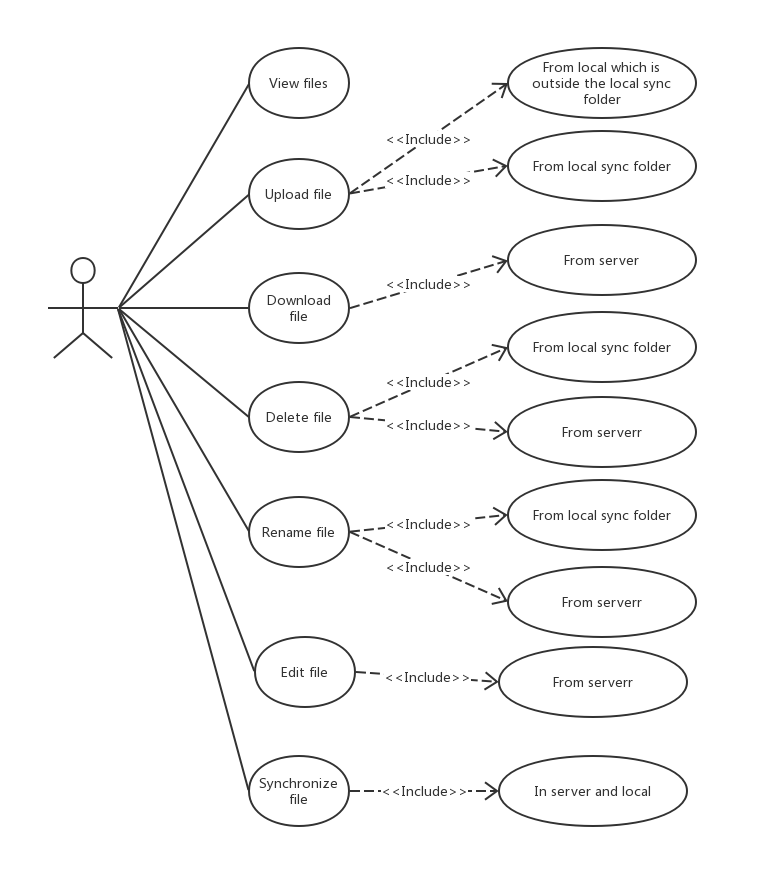
\includegraphics[scale=0.5]{User_use_case.png}

\label{fig:User use case}
\end{minipage}

\subsection{User Sub-scenario Description}
Scenario 1 View files on the server\\\\
Scenario 2 Upload a file from local which is outside the local sync folder\\\\


}


\begin{thebibliography}{9}
\bibitem{Amazon S3}
Amazon S3, [online]Available at:
\texttt{https://docs.aws.amazon.com/AWSJavaScriptSDK/latest/AWS/S3.html}(Accessed: 3 February 2019).

\bibitem{Upload files on S3}
Upload files on S3, [online]Available at:
\texttt{https://blog.csdn.net/qq1147093833/article/details/80267542}(Accessed: 6 February 2019).

\bibitem{Amazon S3}
MyDatahack(2018),'Uploading and Downloading Files in S3 with Node.js'. [online] Available at:
\texttt{https://www.mydatahack.com/uploading-and-downloading-files-in-s3-with-node-js/}(Accessed: 6 February 2019).



\end{thebibliography}






\end{document}
